\documentclass[conference]{IEEEtran}
\IEEEoverridecommandlockouts
% The preceding line is only needed to identify funding in the first footnote. If that is unneeded, please comment it out.

\usepackage{cite}
\usepackage{amsmath,amssymb,amsfonts}
\usepackage{graphicx}
\usepackage{textcomp}
\usepackage{xcolor}
\usepackage{url}
\def\BibTeX{{\rm B\kern-.05em{\sc i\kern-.025em b}\kern-.08em
    T\kern-.1667em\lower.7ex\hbox{E}\kern-.125emX}}

\begin{document}

\title{Development of a Communication-Efficient Edge--Cloud Monitoring System for Wildlife Damage Control in Rural and Mountainous Areas
%\thanks{Identify applicable funding agency here. If none, delete this.}
}

\author{\IEEEauthorblockN{Kota Sato}
\IEEEauthorblockA{\textit{Graduate School of Science and Technology} \\
\textit{Shinshu University}\\
Nagano, Japan \\
25w6039c@shinshu-u.ac.jp}
\and
\IEEEauthorblockN{Shungo Ito}
\IEEEauthorblockA{\textit{Graduate School of Science and Technology} \\
\textit{Shinshu University}\\
Nagano, Japan \\
25w6010e@shinshu-u.ac.jp}
\and
\IEEEauthorblockN{Shimpei Sato}
\IEEEauthorblockA{\textit{Faculty of Engineering} \\
\textit{Shinshu University}\\
Nagano, Japan \\
satos@shinshu-u.ac.jp}
\and
\IEEEauthorblockN{Daisuke Matsuo}
\IEEEauthorblockA{\textit{Organization for IT Initiatives} \\
\textit{Shinshu University}\\
Nagano, Japan \\
daisuke\_matsuo@shinshu-u.ac.jp}
\and
\IEEEauthorblockN{Lin Shan}
\IEEEauthorblockA{\textit{Organization for IT Initiatives} \\
\textit{Shinshu University}\\
Nagano, Japan \\
shanlin@shinshu-u.ac.jp}
}

\maketitle
\vspace{-1.0cm}

\begin{abstract}
Wildlife damage to agricultural crops is a serious issue in rural and mountainous areas of Japan, where continuous monitoring is required under limited communication infrastructure and cost constraints. This paper presents a low-cost and communication-efficient edge--cloud monitoring system using multiple trail cameras for wildlife damage control. The proposed system consists of three layers: edge cameras, an edge server, and a cloud server. Multiple cameras are connected to the edge server through a local area network, enabling communication lines to be aggregated and operational costs to be reduced. To suppress unnecessary image transmission, the system employs a two-stage animal detection process. A lightweight AI model, YOLOv8n, is deployed on the edge server to filter out empty shots caused by environmental factors such as wind and vegetation movement, while a large-scale AI model in the cloud performs final judgment to prevent false alarms. Experimental results show that the proposed system reduced transmitted images by approximately 81.2\% during the daytime and 50.7\% at night, demonstrating its potential as a practical monitoring platform for resilient rural IoT infrastructure.
\end{abstract}

\begin{IEEEkeywords}
Wildlife Monitoring, Edge-Cloud Architecture, Edge AI, Object Detection, Internet of Things (IoT)
\end{IEEEkeywords}

\section{Introduction}
Wildlife damage is a severe problem in Japan, with crop damage reaching 18.8 billion yen in FY2024; thus, wildlife control is an urgent issue \cite{maff}.

Effective countermeasures require an understanding of the time and location of animal appearances, as well as real-time information. Conventionally, wildlife monitoring for this purpose has relied on automatic trail cameras equipped with Passive Infrared Ray (PIR) sensors \cite{Tabak2019,Beery2019,rs18030502}. These devices record images on SD cards for later manual collection. Recently, IoT-based real-time monitoring systems utilizing LTE or satellite communication have emerged to reduce this labor \cite{Whytock2023,Patkar2025,9345858}.

However, large-scale deployment of communication-based cameras faces cost and efficiency challenges. First, PIR sensors often trigger "empty shots" from wind-blown vegetation \cite{Beery2019}. This increases communication traffic and requires manual image sorting. Second, individual LTE contracts and expensive camera units inflate initial and operational costs. Furthermore, existing edge AI cameras consume significant power, requiring bulky solar panels or high-capacity batteries for off-grid operation \cite{Sato2022}. These factors restrict installation locations and act as major barriers for general farmers and local governments.

To address these challenges, approaches such as deep learning for accurate animal detection \cite{10394750,10126065}, empty shot elimination \cite{Tabak2019,Beery2019,VELASCOMONTERO2024102815}, and edge-device power saving \cite{IEICE2020,Sato2022,VELASCOMONTERO2024102815} have been explored. However, the development of systems that balance low-cost real-time notification, empty shot removal, and the integrated operation of numerous low-power cameras has not been sufficiently explored.

In this study, we propose a low-cost, three-layer monitoring system comprising inexpensive edge cameras, an edge server, and a cloud server. In off-grid environments, multiple edge cameras connect to a single edge server via a closed local area network (WLAN). Aggregating communication at the edge server eliminates individual camera contracts, suppressing operational costs. Functionally, edge cameras specialize in image capture, while the edge server handles inference. We adopt a two-stage animal detection process: preliminary filtering by lightweight AI on the edge server, followed by highly accurate final judgment by large-scale AI in the cloud. This role division discards empty shots at the edge to reduce the number of transmitted images, while preventing false alarms via cloud-side verification. Instead of deploying numerous expensive LTE-equipped cameras, adopting this coordinated edge-cloud architecture allows us to construct a monitoring network designed to simultaneously address the reduction of transmitted images, cost suppression, and real-time notification.



\section{Related Work}

The application of deep learning has been a widely noted approach in streamlining wildlife monitoring in recent years. Tabak et al. \cite{Tabak2019} trained Convolutional Neural Networks (CNN) models using a large-scale camera trap image dataset, demonstrating that automatic animal species identification was possible with an accuracy of approximately 98\%. MegaDetector \cite{Beery2019} is a general-purpose object detection model pre-trained on global camera trap images. Fennell et al. \cite{Fennell2022} verified that MegaDetector has a high ability to minimize missed animals and can detect animals in images with high accuracy. Recently, multi-stage approaches combining multiple models have also been proposed, such as using a general-purpose model like MegaDetector to remove empty shot images, followed by another specialized AI to identify animal species \cite{rs18030502,Mulero2025}. This shows that discarding non-target images in the preliminary stage can streamline subsequent processing and confirmation tasks.

Regarding real-time performance, an instant alert system using satellite communication has been developed \cite{Whytock2023}. However, communication costs are extremely high, posing a significant barrier for wide adoption by general farmers and local governments. As attempts to perform edge inference, monitoring systems using single-board computers like Raspberry Pi have been proposed \cite{Patkar2025,Computers2025}. Patkar et al. \cite{Patkar2025} performed animal detection on the edge side using YOLOv8n, demonstrating that inference is possible within practical times even on inexpensive devices. Rahman et al. \cite{Computers2025} showed an approach to reduce duplicate data transmission through tracking processing on the edge side. In recent years, YOLO-based animal intrusion detection systems \cite{10716895,11459678} and tracking systems using PTZ cameras and YOLOv5n \cite{SMC2024} have been proposed. These studies have widely confirmed the effectiveness of edge AI around agricultural lands. Practical applications such as an instant alert system combining PIR sensors and Raspberry Pi \cite{11337723} have also been reported. However, inference-capable single-board computers like Raspberry Pi have relatively high power consumption. Therefore, long-term operation in mountainous areas without commercial power requires large batteries or solar panels. This is a challenge that increases equipment costs and installation difficulty \cite{IEICE2020,Sato2022}.

As an approach to power saving and communication cost reduction, a network architecture consisting of multiple child nodes and one parent node has been proposed \cite{Sato2022}. This method showed the effect of reducing the operational cost and power consumption of the entire system by aggregating communication lines at the parent node. To reduce system costs and communication delays, a hierarchical edge computing approach that delegates main processing to gateway devices like Raspberry Pi has been proposed \cite{8912138}. Furthermore, an IoT architecture linking edge inference with a cloud DB has also been constructed \cite{9345858}. However, even in these methods, edge devices (child nodes) with camera functions often perform detection using deep learning. Therefore, the issue remains that a certain amount of computational resources and power is still required for each of the many deployed camera nodes. In some studies, attempts have been made to lower system power consumption by utilizing power-saving microcontrollers \cite{IEICE2020}. However, due to processing performance constraints, challenges in real-time performance remain, or verifications are often limited to small-scale configurations. The construction of a communication network assuming multiple deployments in an actual field environment and the practical filtering effect of empty shot images have not yet been sufficiently verified.

Furthermore, in recent years, research on wildlife damage control has progressed beyond image-based detection to more active countermeasures. For example, a capture system that recognizes troops of monkeys using deep learning and remotely activates traps has been developed \cite{8716170}. Also, a system that repels animals by emitting specific ultrasonic waves according to the detected animal species has been proposed \cite{11324419}. The low-cost communication-based monitoring system proposed in this study is expected to cooperate with these advanced damage deterrence and capture systems in the future. As a result, it is considered applicable as a sensor network supporting operations in extensive agricultural lands.


\section{Proposed System}
As described in Section II, deploying conventional monitoring systems in multiple field environments faces challenges regarding power consumption, computational resource constraints of edge devices, and the practical filtering of empty shot images. To overcome these challenges, this study applies the concept of line aggregation by Sato et al. \cite{Sato2022} and proposes a three-tier low-cost communication-based monitoring system. This system consists of power-saving edge cameras dedicated solely to photography, an edge server responsible for inference and communication, and a cloud server handling data post-processing and notification.

Edge cameras do not perform inference processing; instead, they specialize in image acquisition using power-saving microcontrollers capable of long-term operation without solar panels. By aggregating images from multiple cameras into a single edge server, individual communication contracts for each camera are eliminated, suppressing the system's operational costs. Additionally, this system adopts a two-stage processing architecture. Preliminary filtering is performed by lightweight AI on the edge server to extract potential animal images, followed by highly accurate re-evaluation and notification by large-scale AI on the cloud side. This two-stage processing enables role division across layers: discarding empty shots at the edge reduces the number of transmitted images, while accurate cloud-side judgment prevents false alarms during immediate notifications. Through these approaches, we realize a system designed to simultaneously address real-time performance, empty shot removal, reduction in the number of transmitted images, and operational cost suppression.

This section describes the architecture and detailed processing flow of the proposed system.

\subsection{System Architecture}
The overall configuration of the proposed system is shown in Fig.~\ref{fig:system}. This system consists of the following three main nodes and the network connecting them:
\begin{enumerate}
    \item \textbf{Edge Camera}: Image acquisition and transfer to the edge server.
    \item \textbf{Edge Server}: Image aggregation, primary selection by lightweight AI, and transfer to the cloud server.
    \item \textbf{Cloud Server}: Re-evaluation by large-scale AI, data accumulation, and user notification.
    \item \textbf{Network Configuration}: Construction of communication paths between edges and the cloud.
\end{enumerate}

\begin{figure}[tb]
    \centerline{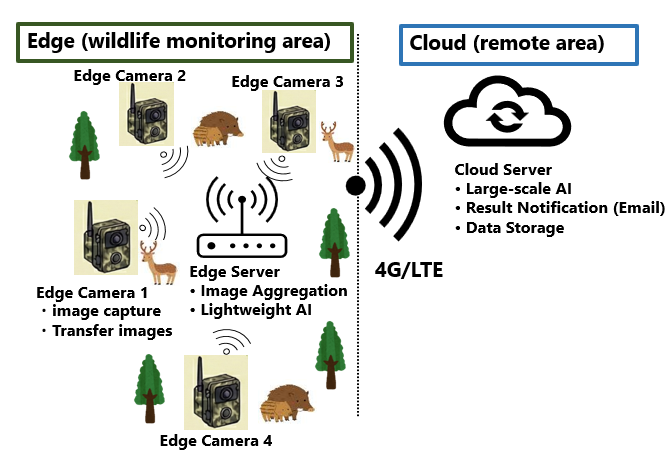
\includegraphics[width=0.8\linewidth]{../img/system_structure_eng.png}}
    \caption{Overall architecture of the proposed system.}
    \label{fig:system}
\end{figure}

\subsubsection{Edge Camera}
Edge cameras are deployed directly throughout the monitoring area. They are responsible for detecting the appearance of animals, capturing images, and transferring them to the edge server via local communication. Since they are intended to be deployed in large numbers in outdoor environments without commercial power, they must utilize ultra-low-power microcontrollers and be capable of operating for long periods solely on independent batteries.

In the implementation of this paper, we adopted the XIAO ESP32S3 Sense manufactured by Seeed Studio as the device. Although inexpensive, this device has Wi-Fi communication and camera functions. Furthermore, its Deep Sleep function minimizes power consumption during standby, aiming to fulfill the requirement for long-term operation. A PIR sensor is used as a trigger for motion detection, and HTTP communication via Wi-Fi is used to transmit images to the edge server. It uses eight AA batteries (6V) as a power source, facilitating installation in locations without power infrastructure. Fig.~\ref{fig:camera} shows an overview of the edge camera prototype.

\begin{figure}[tb]
    \centerline{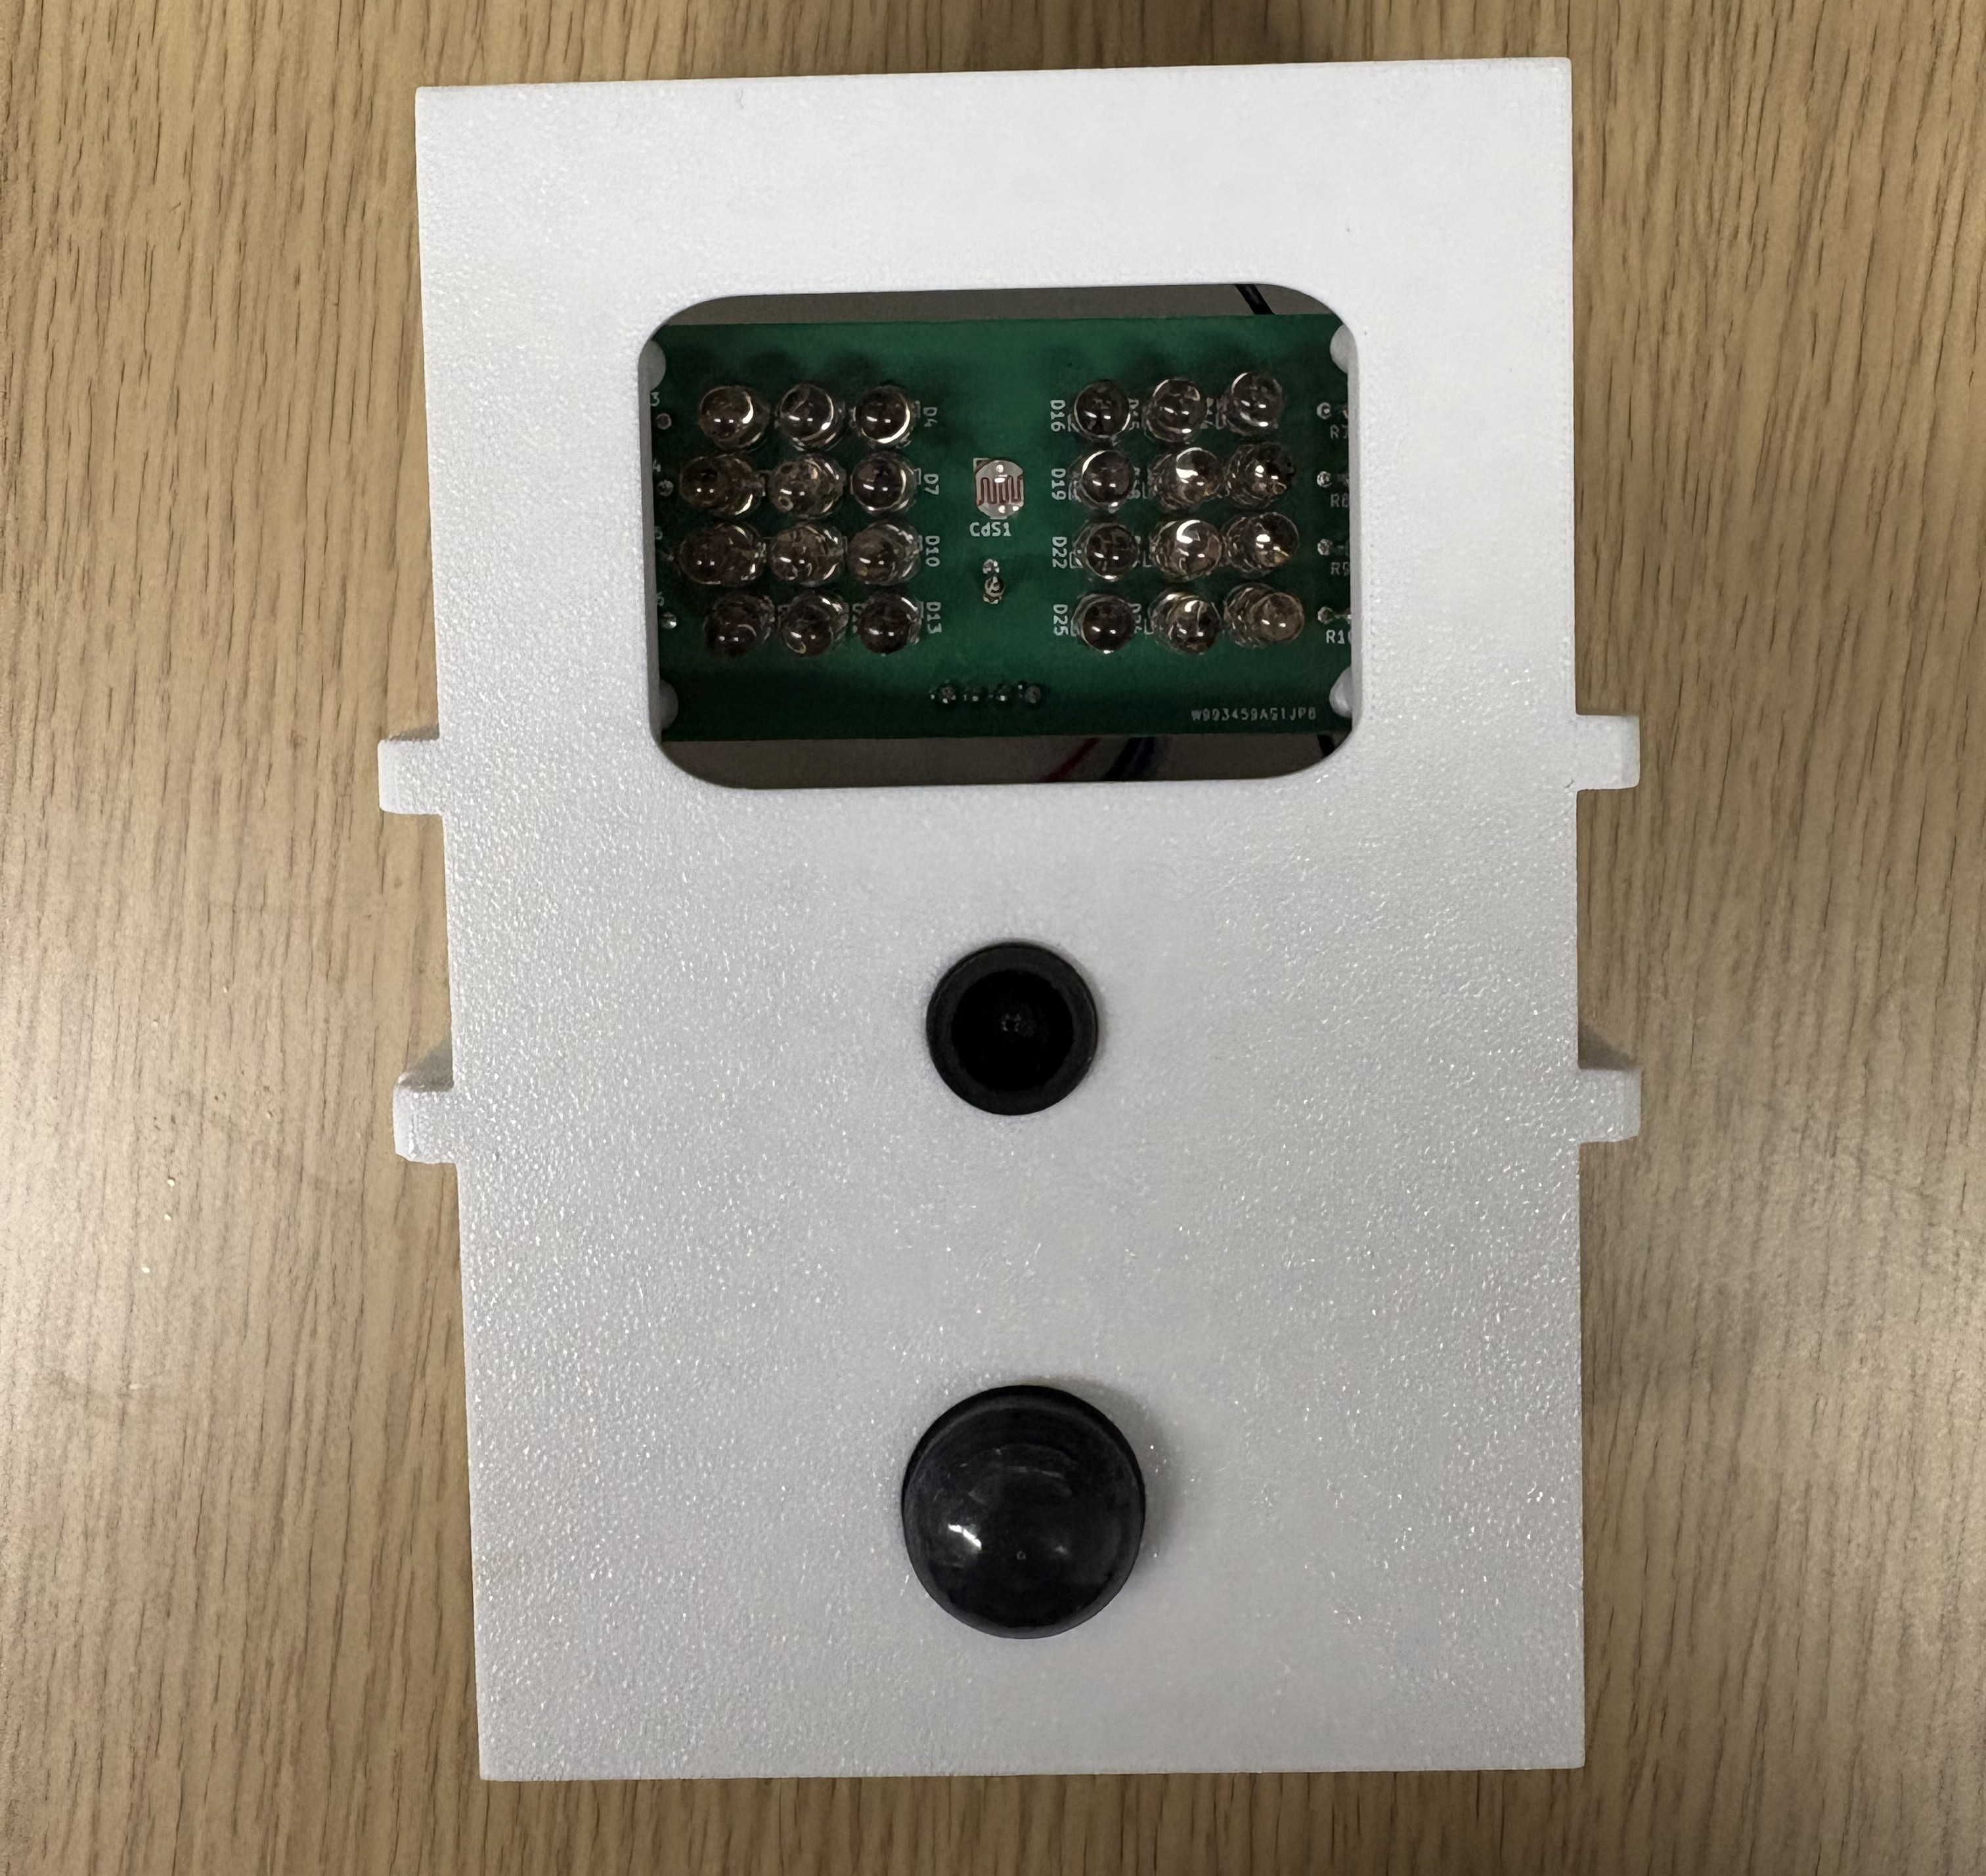
\includegraphics[width=0.45\linewidth]{../img/prototype_camera.jpeg}}
    \caption{Prototype of the edge camera.}
    \label{fig:camera}
\end{figure}

\subsubsection{Edge Server}
The edge server functions as a hub connecting multiple edge cameras and is responsible for reducing operational costs by aggregating communication lines. Simultaneously, it executes primary selection using lightweight AI at the edge to discard empty shot images and transfer only images containing animals, significantly reducing the number of images transmitted to the cloud. To perform these processes autonomously in outdoor environments, the small computer and communication module must be capable of continuous operation using solar panels or similar power sources.

In our implementation, a Raspberry Pi 4B is used as the small computer, and an NEC Aterm HT100LN is used as the communication module. For the lightweight AI used for primary selection, we adopted YOLOv8n, pre-trained on the COCO dataset, which can perform inference at practical speeds even on devices with limited computational resources like the Raspberry Pi, while maintaining sufficient detection accuracy. HTTP communication is also used for transferring images to the cloud server. To operate this configuration continuously in an environment without commercial power, power equipment consisting of an approximately 200W solar panel and a 100Ah large-capacity battery is required based on estimates.

\subsubsection{Cloud Server}
The cloud server performs re-evaluation on images that passed the primary selection using a large-scale AI model, utilizing its abundant computational resources. This ensures accurate final determination of animal presence to prevent false alarms while immediately notifying the user when target animals are detected. In addition, it acts as a platform to centrally store received image data regardless of the judgment result, aiding future analysis or AI retraining.

In our implementation, MegaDetector v5a is used as the large-scale AI model. MegaDetector is a pre-trained object detection model using images captured in diverse environments globally and achieves high accuracy in animal detection, thus realizing reliable re-evaluation on the cloud server.

\subsubsection{Network Configuration}
Communication between devices in this system adopts a two-stage network configuration that considers operational costs and environmental constraints. The first stage is local communication between the edge cameras and the edge server. To prevent the increase in operational costs caused by contracting communication lines for each of the many edge cameras deployed in the monitoring area, a local network (WLAN) is built using a Wi-Fi access point installed on the edge server side. This aggregates images from multiple cameras to the edge server once, making individual communication contracts for cameras unnecessary. The second stage is wide-area communication from the edge server to the cloud server. Using an LTE communication module connected to the edge server, only images that passed the primary selection are transmitted to the cloud server via HTTP communication over the internet. This hierarchical network configuration realizes a mechanism to minimize communication costs while maintaining network scalability.

In our implementation, the aforementioned NEC Aterm HT100LN is adopted as the core communication equipment to construct these networks. This device is connected to the edge server, utilizing its 2.4GHz Wi-Fi access point function to construct a local communication network with the edge cameras, while establishing a connection to the cloud using its LTE communication function.

\subsection{Data Processing Flow}
The data processing flow of the proposed system is shown in Fig.~\ref{fig:flow}. The layers cooperate to execute stages from image acquisition at the edge camera to primary selection at the edge server, and re-evaluation and notification at the cloud server. The processing flow of each component is described below.

\begin{figure}[tb]
    \centerline{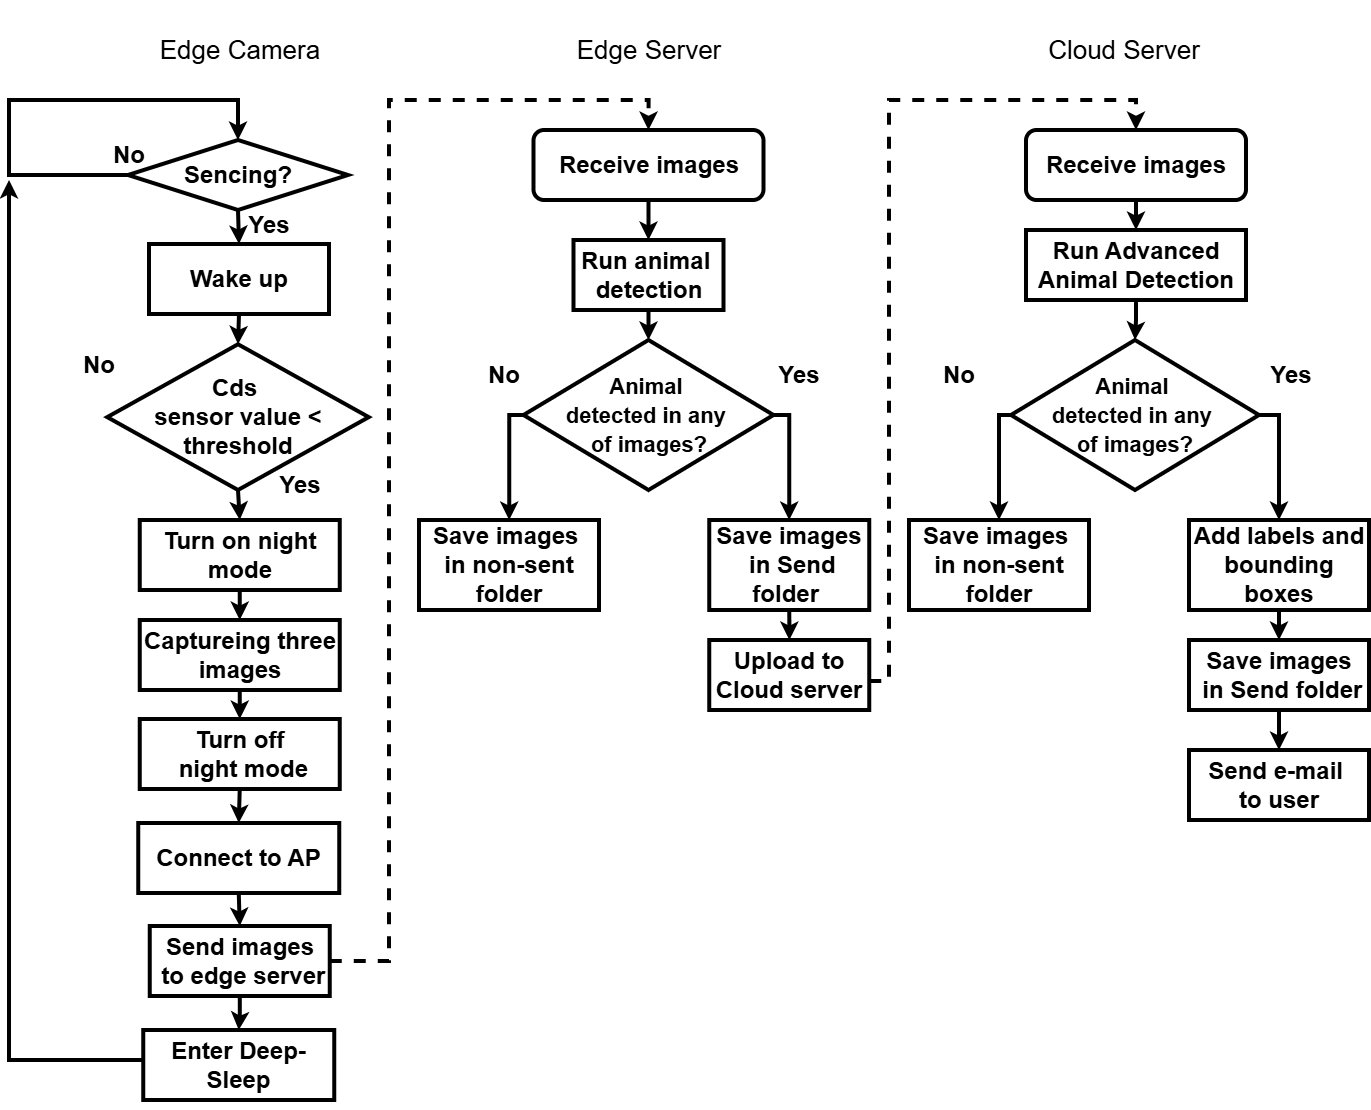
\includegraphics[width=\columnwidth]{../img/system_flow_eng.png}}
    \caption{Data processing flow of the proposed system.}
    \label{fig:flow}
\end{figure}

\subsubsection{Edge Camera Processing Flow}
The edge camera maintains a standby state using Deep Sleep mode and wakes up the moment the PIR sensor detects a heat source. After waking up, it captures three consecutive images in burst mode and immediately transmits them to the edge server via HTTP communication. After transmission is complete, the edge camera returns to the standby state after a certain interval, minimizing battery consumption.

\subsubsection{Edge Server Processing Flow}
The edge server constantly awaits image reception from edge cameras. Upon receiving images, it executes primary inference using YOLOv8n. If a class corresponding to an animal is detected in at least one of the three received images, the images are moved to a storage directory and transferred to the cloud server. If no animal is detected (e.g., empty shots due to swaying vegetation), the images are not transmitted, reducing the frequency of image transmissions.

\subsubsection{Cloud Server Processing Flow}
The cloud server constantly awaits transfers from the edge server. Upon receiving images, it re-detects animals using MegaDetector, a large-scale AI. Only when target animals are detected, it notifies the user of the appearance via email along with the image. Regardless of the judgment result, the images transferred from the edge server and the analysis results are accumulated in cloud storage. If no animal is detected, the system only accumulates the data and does not notify the user.

\section{Experimental Results}
In this section, we describe the following four experiments conducted to verify the practicality of the proposed system:
\begin{enumerate}
    \item Measurement of power consumption during operation of each node.
    \item Evaluation of communication performance in an outdoor line-of-sight environment.
    \item Verification of object detection accuracy using a dataset collected in Kiso Town, Nagano Prefecture.
    \item Measurement of system processing time.
\end{enumerate}

\subsection{Experimental Environment and Parameters}
The equipment configuration used for the experiments is shown in Table \ref{tab:components}. Communication tests between the edge camera and the edge server were conducted in a line-of-sight outdoor environment on a sunny day.

\begin{table}[tb]
    \caption{System Components}
    \label{tab:components}
    \vspace{-0.2cm}
    \begin{center}\footnotesize
    \scalebox{0.85}{
    \begin{tabular}{|l|l|l|}
        \hline
        \textbf{Component} & \textbf{Model} & \textbf{Remarks} \\
        \hline \hline
        \multicolumn{3}{|l|}{\textbf{Edge Camera}} \\
        \hline
        Main Unit & Seeed Studio XIAO ESP32S3 Sense & Microcontroller with Wi-Fi/Camera \\
        \hline
        PIR Sensor & Panasonic PaPIRs & Detection range $\sim$14m \\
        \hline
        Power Supply & 8 $\times$ AA batteries & 6V \\
        \hline \hline
        \multicolumn{3}{|l|}{\textbf{Edge Server}} \\
        \hline
        Main Unit & Raspberry Pi 4B & 4GB RAM \\
        \hline
        Power Supply & Recommended (Est.) & $\sim$200W panel, 100Ah battery \\
        \hline
        Comms Module & NEC Aterm HT100LN & LTE router \\
        \hline
    \end{tabular}
    }
    \end{center}
    \vspace{-0.4cm}
\end{table}

\subsection{Power Consumption Evaluation of Edge Camera}
Because this system assumes operation in agricultural and mountainous areas where commercial power is difficult to access, the power consumption of each node is a critical indicator determining practicality. We measured the power consumption of the edge camera in each operating state (Table \ref{tab:camera_power}). At a power supply voltage of 5.0V, the current during standby was 114mA, and the maximum peak current during startup was 946mA.

\begin{table}[tb]
    \caption{Power Consumption of Edge Camera (5.0V)}
    \label{tab:camera_power}
    \vspace{-0.2cm}
    \begin{center}\footnotesize
    \scalebox{0.85}{
    \begin{tabular}{|l|r|r|}
        \hline
        \textbf{Operating State} & \textbf{Current (mA)} & \textbf{Power (W)} \\
        \hline \hline
        Standby & 114 & 0.57 \\
        \hline
        Startup (Peak) & 946 & 4.73 \\
        \hline
        Wi-Fi Transmission & 250 & 1.25 \\
        \hline
    \end{tabular}
    }
    \end{center}
    \vspace{-0.4cm}
\end{table}

\subsection{Power Consumption Evaluation of Edge Server}
We similarly measured the power consumption of the edge server (Raspberry Pi 4B). At 5.0V, the idle current consumption was 405$\sim$410mA (approx. 2.05W). Adding the maximum power consumption of the LTE router (approx. 6W), the total power consumption of the edge server is approximately 8W.

\subsection{WLAN Communication Performance}
Under a line-of-sight environment, we evaluated communication stability while varying the distance between the edge camera and the server. Table \ref{tab:comm_perf} shows the experimental results. At close range (approx. 1m), RSSI remained stable at around -30$\sim$-35dBm. At a distance of 100m, RSSI was around -60$\sim$-65dBm, and it dropped to -77$\sim$-80dBm at the maximum distance of 200m. While connection establishment and image transfer were successfully completed without problems up to 100m, approaching the 200m point caused RSSI to fall below -75dBm, resulting in noticeable latency and communication instability. Thus, in this configuration, stable image transfer is achieved up to approximately 100m in a line-of-sight environment, while communication quality degrades near 200m, suggesting that repeaters or alternative communication methods are necessary for stable operation over longer distances.

\begin{table}[tb]
    \caption{Communication Performance (Line-of-Sight Environment)}
    \label{tab:comm_perf}
    \vspace{-0.2cm}
    \begin{center}\footnotesize
    \scalebox{0.85}{
    \begin{tabular}{|c|c|}
        \hline
        \textbf{Distance (m)} & \textbf{RSSI (dBm)} \\
        \hline \hline
        $\approx$ 1 & -30 $\sim$ -35 \\
        \hline
        $\approx$ 100 & -60 $\sim$ -65 \\
        \hline
        $\approx$ 200 & -77 $\sim$ -80 \\
        \hline
    \end{tabular}
    }
    \end{center}
    \vspace{-0.4cm}
\end{table}

\subsection{Reduction in the Number of Transmitted Images by Edge Server}
We evaluated the object detection accuracy using YOLOv8 on the edge server and the resulting reduction in the number of transmitted images. We evaluated YOLOv8n on the edge server using images from Kiso Town (June-November 2025). MegaDetector v5a served as the reference labels (Table \ref{tab:ai_accuracy}). To minimize missed animals (unintended image discarding) during the primary selection, the judgment threshold for YOLOv8n was intentionally set low at 0.05. This evaluation uses MegaDetector outputs as reference labels. Therefore, the accuracy indicates agreement with MegaDetector, not absolute performance against ground-truth. Precision is the proportion of true animal images among AI detections. Recall is the proportion of detected animals among actual animal images. Ref(MD) in the table represents the reference labels by MegaDetector.

\begin{table}[tb]
    \caption{AI Detection Accuracy (Threshold: 0.05)}
    \label{tab:ai_accuracy}
    \vspace{-0.2cm}
    \begin{center}\footnotesize
    \scalebox{0.85}{
    \begin{tabular}{|c|c|r|r|r|r|}
        \hline
        \multicolumn{2}{|c|}{\textbf{}} & \multicolumn{2}{c|}{\textbf{Daytime (YOLOv8n)}} & \multicolumn{2}{c|}{\textbf{Nighttime (YOLOv8n)}} \\
        \cline{3-6}
        \multicolumn{2}{|c|}{\textbf{}} & \makebox[1.2cm][c]{\textbf{Pos.}} & \makebox[1.2cm][c]{\textbf{Neg.}} & \makebox[1.2cm][c]{\textbf{Pos.}} & \makebox[1.2cm][c]{\textbf{Neg.}} \\
        \hline \hline
        \textbf{Ref} & \textbf{True} & \textbf{195} & 13 & \textbf{104} & 48 \\
        \cline{2-6}
        \textbf{(MD)} & \textbf{False} & 73 & \textbf{1,147} & 28 & \textbf{88} \\
        \hline \hline
        \multicolumn{2}{|c|}{\textbf{Precision}} & \multicolumn{2}{c|}{72.8\%} & \multicolumn{2}{c|}{78.8\%} \\
        \hline
        \multicolumn{2}{|c|}{\textbf{Recall}} & \multicolumn{2}{c|}{93.8\%} & \multicolumn{2}{c|}{68.4\%} \\
        \hline
    \end{tabular}
    }
    \end{center}
    \vspace{-0.4cm}
\end{table}

The AI object detection accuracy resulted in a recall of 93.8\% and precision of 72.8\% during the daytime. Conversely, at night, the recall was 68.4\% and the precision was 78.8\%, showing a tendency for recall to decrease compared to daytime.

Next, Table \ref{tab:comm_reduction} shows the image reduction rate. The image reduction rate represents the proportion of events where the server judged "transmission unnecessary (no animal)" out of the total number of triggers (the number of times the PIR sensor reacted). In this evaluation, the three images captured per PIR trigger are treated as one cycle.

\begin{equation}
    \text{Reduction} = \left( 1 - \frac{\text{Transmitted Triggers}}{\text{Total Triggers}} \right) \times 100 \label{eq:reduction}
\end{equation}

\begin{table}[tb]
    \caption{Image Reduction Rate by Day/Night}
    \label{tab:comm_reduction}
    \vspace{-0.2cm}
    \begin{center}\footnotesize
    \scalebox{0.85}{
    \begin{tabular}{|l|r|r|}
        \hline
        \textbf{Item} & \textbf{Nighttime} & \textbf{Daytime} \\
        \hline \hline
        Total Triggers & 268 & 1,428 \\
        \hline
        Transmitted Triggers & 132 & 268 \\
        \hline
        Reduction Rate (\%) & 50.7 & 81.2 \\
        \hline
    \end{tabular}
    }
    \end{center}
    \vspace{-0.4cm}
\end{table}

As a result, the image reduction rate was 81.2\% during the daytime and 50.7\% at night, confirming a tendency for the reduction rate to be lower at night than during the day.

\subsection{Total System Processing Time}
We measured the overall system processing time in a stable communication environment with an RSSI of around -35dBm. The processing time on the edge side (from camera capture to completion of transmission processing at the edge server) was approximately 33 seconds (total of approx. 20 seconds for camera processing and approx. 13 seconds for edge server processing). The processing on the cloud side (from reception to completion of email notification) required approximately 11 seconds. As a result, the total time required from detecting an animal to completing an email notification to the user was approximately 44 seconds.

\section{Discussion}

In the experiment, image reduction rates of 81.2\% during the daytime and 50.7\% at night were achieved. This is because empty shots caused by wind and temperature changes were appropriately excluded on the edge side. This demonstrated that the overall number of transmitted images can be suppressed. On the other hand, the recall at night was low at 68.4\%. The limitations of the lightweight model and the low image quality at night are considered the primary factors. To prevent missed detections in wildlife damage control, it is necessary to improve accuracy, such as through model training specialized for night images. Furthermore, it was estimated that the edge camera's battery would be depleted in approximately 35 hours even in the standby state alone. With the current configuration, practical long-term operation cannot be expected even using eight AA batteries. The main cause of this increase in standby current consumption is considered to be the power supply control to the SD card module. Towards power saving, it is necessary to review the hardware design and implement appropriate power supply control.

\section{Conclusion}
We proposed a low-cost monitoring system for wildlife damage control. It uses a three-layer structure: edge cameras, an edge server, and a cloud server. This reduces costs and workload. We proposed an architecture that aggregates multiple cameras into a single line via a local network, eliminating individual contracts and suppressing operational costs. Our verification experiments combined primary selection (YOLOv8n) and cloud re-judgment. We confirmed image reduction rates of 81.2\% during the daytime and 50.7\% at night.

In the future, we plan to improve the detection model for night images, control the power supply of the SD card module, and review the intermittent operation and power configuration of the edge server to enhance long-term operability in actual environments. Furthermore, we will consider the introduction of LPWA (Low Power Wide Area) communication to expand the monitoring area and ensure communication stability in environments with many obstacles. In addition, we aim to improve the reduction and recall rates through transfer learning of the AI model on the edge side. We will also consider implementing an animal species discrimination function on the cloud side and building a web interface for users. Through these efforts, we will continue to expand functions to enhance the practicality and convenience of the system.



\section*{Acknowledgment}

This research and development work was supported by the Ministry of Internal Affairs and Communications (MIC), Japan, awarded through the FORWARD program under grant \#JPMI250420001 (Principal Investigator: Lin Shan).

\bibliographystyle{IEEEtran}
\bibliography{refs_english}

\end{document}
